% Options for packages loaded elsewhere
\PassOptionsToPackage{unicode}{hyperref}
\PassOptionsToPackage{hyphens}{url}
\documentclass[
]{article}
\usepackage{xcolor}
\usepackage{amsmath,amssymb}
\setcounter{secnumdepth}{-\maxdimen} % remove section numbering
\usepackage{iftex}
\ifPDFTeX
  \usepackage[T1]{fontenc}
  \usepackage[utf8]{inputenc}
  \usepackage{textcomp} % provide euro and other symbols
\else % if luatex or xetex
  \usepackage{unicode-math} % this also loads fontspec
  \defaultfontfeatures{Scale=MatchLowercase}
  \defaultfontfeatures[\rmfamily]{Ligatures=TeX,Scale=1}
\fi
\usepackage{lmodern}
\ifPDFTeX\else
  % xetex/luatex font selection
\fi
% Use upquote if available, for straight quotes in verbatim environments
\IfFileExists{upquote.sty}{\usepackage{upquote}}{}
\IfFileExists{microtype.sty}{% use microtype if available
  \usepackage[]{microtype}
  \UseMicrotypeSet[protrusion]{basicmath} % disable protrusion for tt fonts
}{}
\makeatletter
\@ifundefined{KOMAClassName}{% if non-KOMA class
  \IfFileExists{parskip.sty}{%
    \usepackage{parskip}
  }{% else
    \setlength{\parindent}{0pt}
    \setlength{\parskip}{6pt plus 2pt minus 1pt}}
}{% if KOMA class
  \KOMAoptions{parskip=half}}
\makeatother
\usepackage{graphicx}
\makeatletter
\newsavebox\pandoc@box
\newcommand*\pandocbounded[1]{% scales image to fit in text height/width
  \sbox\pandoc@box{#1}%
  \Gscale@div\@tempa{\textheight}{\dimexpr\ht\pandoc@box+\dp\pandoc@box\relax}%
  \Gscale@div\@tempb{\linewidth}{\wd\pandoc@box}%
  \ifdim\@tempb\p@<\@tempa\p@\let\@tempa\@tempb\fi% select the smaller of both
  \ifdim\@tempa\p@<\p@\scalebox{\@tempa}{\usebox\pandoc@box}%
  \else\usebox{\pandoc@box}%
  \fi%
}
% Set default figure placement to htbp
\def\fps@figure{htbp}
\makeatother
\ifLuaTeX
  \usepackage{luacolor}
  \usepackage[soul]{lua-ul}
\else
  \usepackage{soul}
\fi
\setlength{\emergencystretch}{3em} % prevent overfull lines
\providecommand{\tightlist}{%
  \setlength{\itemsep}{0pt}\setlength{\parskip}{0pt}}
\usepackage{bookmark}
\IfFileExists{xurl.sty}{\usepackage{xurl}}{} % add URL line breaks if available
\urlstyle{same}
% fallback for those not using the hyperref driver hyperxmp:
\makeatletter
\@ifundefined{xmpquote}{\newcommand{\xmpquote}[1]{#1}}{}
\makeatother
\hypersetup{
  hidelinks,
  pdfcreator={LaTeX via pandoc}}

\author{}
\date{}

\begin{document}

\begin{quote}
\textbf{PROYECTO FINAL DE INGENIERÍA}

\textbf{INFRAEYE}

\textbf{Bianchi Canelo, Máximo -- LU1156650}

Ingeniería en Informática

\textbf{Rodriguez Costantini, Ignacio -- LU1153276}

Ingeniería en Informática

Tutor:

\textbf{Foglino, Alejandro Luis, UADE}

\textbf{Junio 13, 2026}
\end{quote}

\includegraphics[width=1.13476in,height=1.11375in,alt={logo+v}]{media/image1.jpg}

\begin{quote}
\textbf{UNIVERSIDAD ARGENTINA DE LA EMPRESA}

FACULTAD DE INGENIERÍA Y CIENCIAS EXACTAS
\end{quote}

\textbf{Tabla de contenido}

\hyperref[introducciuxf3n]{\textbf{1. Introducción 4}}

\begin{quote}
\hyperref[objetivos]{1.1. Objetivos 6}

\hyperref[objetivo-general]{1.1.1. Objetivo General 6}

\hyperref[objetivos-especuxedficos]{1.1.2. Objetivos Específicos 6}
\end{quote}

\hyperref[marco-teuxf3rico]{\textbf{2. Marco Teórico 7}}

\begin{quote}
\hyperref[computaciuxf3n-en-la-nube-cloud-computing]{2.1. Computación en
la nube (Cloud Computing) 7}

\hyperref[definiciuxf3n-de-computaciuxf3n-en-la-nube]{2.1.1. Definición
de computación en la nube 7}

\hyperref[caracteruxedsticas-principales]{2.1.1.1. Características
principales 7}

\hyperref[modelos-de-servicio]{2.1.2. Modelos de servicio 8}

\hyperref[modelos-de-despliegue]{2.1.3. Modelos de despliegue 8}

\hyperref[arquitectura-y-administraciuxf3n-de-infraestructura-cloud]{2.2.
Arquitectura y administración de infraestructura cloud 8}

\hyperref[concepto-de-infraestructura-cloud]{2.2.1. Concepto de
infraestructura cloud 8}

\hyperref[administraciuxf3n-de-infraestructura-cloud]{2.2.2.
Administración de infraestructura cloud 9}

\hyperref[escalabilidad-y-elasticidad]{2.3. Escalabilidad y elasticidad
9}

\hyperref[monitoreo]{2.4. Monitoreo 10}

\hyperref[concepto-de-monitoreo]{2.4.1. Concepto de monitoreo 10}

\hyperref[observabilidad]{2.5. Observabilidad 11}

\hyperref[gestiuxf3n-y-optimizaciuxf3n-de-costos-cloud]{2.6. Gestión y
optimización de costos cloud 12}

\hyperref[infrastructure-as-code-iac]{2.7. Infrastructure as Code (IaC)
13}

\hyperref[concepto-de-infrastructure-as-code]{2.7.1. Concepto de
Infrastructure as Code 13}

\hyperref[terraform]{2.7.2. Terraform 13}

\hyperref[machine-learning-aplicado-a-infraestructura-cloud]{2.8.
Machine Learning aplicado a infraestructura cloud 14}

\hyperref[concepto-de-machine-learning]{2.8.1. Concepto de Machine
Learning 14}

\hyperref[aprendizaje-supervisado-y-no-supervisado]{2.8.2. Aprendizaje
supervisado y no supervisado 14}

\hyperref[algoritmo-isolation-forest]{2.9. Algoritmo Isolation Forest
14}

\hyperref[interfaces-gruxe1ficas-y-visualizaciuxf3n-de-datos]{2.10.
Interfaces gráficas y visualización de datos 15}

\hyperref[devops-y-automatizaciuxf3n]{2.11. DevOps y Automatización 16}

\hyperref[concepto-de-devops]{2.11.1. Concepto de DevOps 16}

\hyperref[automatizaciuxf3n-de-procesos]{2.11.2. Automatización de
procesos 16}

\hyperref[integraciuxf3n-entre-automatizaciuxf3n-y-monitoreo]{2.11.3.
Integración entre automatización y monitoreo 17}
\end{quote}

\hyperref[estado-del-arte]{\textbf{3. Estado del Arte 18}}

\begin{quote}
\hyperref[soluciones-comerciales-vigentes]{3.1. Soluciones Comerciales
Vigentes 18}

\hyperref[amazon-cloudwatch-y-aws-cost-explorer]{3.1.1. Amazon
CloudWatch y AWS Cost Explorer 18}

\hyperref[google-cloud-operations-suite]{3.1.2. Google Cloud Operations
Suite 19}

\hyperref[azure-monitor-y-azure-advisor]{3.1.3. Azure Monitor y Azure
Advisor 20}

\hyperref[huawei-cloud-eye-y-huawei-cloud-cost-center]{3.1.4. Huawei
Cloud Eye y Huawei Cloud Cost Center 21}

\hyperref[vmware-cloudhealth]{3.1.5. VMware CloudHealth 23}

\hyperref[soluciones-de-cuxf3digo-abierto]{3.2. Soluciones de Código
Abierto 23}

\hyperref[prometheus]{3.2.1. Prometheus 24}

\hyperref[grafana]{3.2.2. Grafana 24}

\hyperref[opentelemetry]{3.2.3. OpenTelemetry 24}

\hyperref[anuxe1lisis-comparativo]{3.3. Análisis Comparativo 25}
\end{quote}

\hyperref[bibliografuxeda]{\textbf{4. Bibliografía 27}}

\hyperref[anexo-a]{\textbf{5. Anexo A 32}}

\section{Introducción}\label{introducciuxf3n}

\begin{quote}
La transformación digital ha modificado sustancialmente la forma en que
las organizaciones gestionan sus recursos tecnológicos. En las últimas
décadas, la dependencia de sistemas informáticos ha crecido
exponencialmente, convirtiendo a la tecnología en un pilar fundamental
para la operación empresarial. Según Gartner, para 2025, más del 85\% de
las organizaciones adoptarán modelos centrados en la nube como principio
rector de su arquitectura tecnológica (GARTNER, 2025).

La computación en la nube surge como respuesta a la necesidad de
flexibilidad y eficiencia en el acceso a recursos tecnológicos. Este
paradigma permite provisionar infraestructura, plataformas y servicios
bajo demanda, eliminando la necesidad de inversiones iniciales
significativas en hardware físico. El National Institute of Standards
and Technology (NIST) define cloud computing como "un modelo para
permitir acceso conveniente, bajo demanda y ubicuo a un pool compartido
de recursos computacionales configurables que pueden ser rápidamente
provisionados y liberados con mínimo esfuerzo de gestión o interacción
con el proveedor de servicio" (MELL, Peter; 2011).

Las características fundamentales de la computación en la nube incluyen
elasticidad, disponibilidad bajo demanda, pooling de recursos, medición
de servicios y acceso amplio a través de la red. Estas propiedades
permiten a las organizaciones escalar recursos vertical y
horizontalmente según las necesidades operativas, optimizando tanto el
rendimiento como los costos asociados. Sin embargo, esta flexibilidad
introduce complejidades en la gestión que no estaban presentes en
modelos tradicionales de infraestructura estática. Como señala Buyya et
al., "la naturaleza dinámica y elástica de las aplicaciones cloud y la
provisionamiento de recursos en entornos heterogéneos y geográficamente
distribuidos presenta desafíos significativos para el manejo eficiente
de recursos" (BUYYA, Rajkumar; 2013).

La gestión de costos en entornos cloud representa uno de los principales
desafíos operativos. El modelo de pago por uso, aunque económicamente
ventajoso en teoría, puede resultar en gastos impredecibles sin
mecanismos adecuados de monitoreo y control. Un estudio de Flexera
revela que las organizaciones desperdician aproximadamente el 32\% de su
gasto en cloud debido a recursos subutilizados y sobredimensionados
(FLEXERA, 2023). Esta situación evidencia la necesidad de herramientas
que proporcionen visibilidad granular sobre el consumo de recursos y
faciliten la identificación de ineficiencias.

La complejidad de las arquitecturas cloud modernas, caracterizadas por
microservicios, contenedores y múltiples niveles de abstracción,
dificulta la detección manual de anomalías en el consumo. Los
responsables técnicos enfrentan el desafío de identificar instancias
sobredimensionadas, recursos ociosos, configuraciones subóptimas y
patrones de uso ineficientes. Según Amazon Web Services, "la
optimización continua de costos requiere un enfoque sistemático que
combine monitoreo automatizado, análisis de datos y procesos de
gobernanza" (AWS, 2023).

La automatización de infraestructura ha evolucionado como respuesta a
estas complejidades. La práctica conocida como Infraestructura como
Código (Infrastructure as Code - IaC) permite definir, desplegar y
gestionar recursos tecnológicos mediante archivos de configuración
versionables y reproducibles. Morris define IaC como "la práctica de
gestionar y provisionar recursos de infraestructura a través de archivos
de configuración definidos por máquina, en lugar de herramientas
interactivas o scripts manuales" (MORRIS, Kief; 2016). Terraform,
desarrollado por HashiCorp, se ha consolidado como una de las
herramientas más adoptadas para IaC, permitiendo gestionar
infraestructura multi-cloud mediante un lenguaje declarativo.

El aprendizaje automático ofrece nuevas posibilidades para abordar la
complejidad del análisis de infraestructura cloud. Las técnicas de
machine learning, particularmente los algoritmos no supervisados,
permiten identificar patrones anómalos en grandes volúmenes de datos
operativos sin requerir etiquetado previo. El algoritmo Isolation
Forest, propuesto por Liu et al. en 2008, detecta anomalías mediante el
aislamiento de observaciones a través de particiones recursivas,
resultando especialmente efectivo para detectar outliers en datasets
multidimensionales (LIU; TING; ZHOU, 2008). Esta técnica resulta
particularmente adecuada para identificar comportamientos anómalos en
métricas de infraestructura, donde las ineficiencias se manifiestan como
desviaciones respecto a patrones normales de operación.

En este contexto, el presente proyecto propone el diseño y desarrollo de
una plataforma integrada para el monitoreo y optimización de recursos en
entornos cloud. La solución combina tres pilares fundamentales: primero,
la recolección sistemática de métricas operativas que proporcionen
visibilidad sobre el estado y consumo de recursos; segundo, la
aplicación del algoritmo Isolation Forest para detectar ineficiencias y
comportamientos anómalos; y tercero, la generación de recomendaciones
accionables orientadas a mejorar la utilización de recursos y optimizar
costos. Adicionalmente, se incorpora una interfaz gráfica para
visualización de datos y un módulo de despliegue automatizado basado en
Terraform.

El desarrollo se enfoca en un prototipo funcional integrado con
servicios cloud de Huawei, orientado a validar la viabilidad técnica de
la propuesta en un entorno controlado. La selección de Huawei Cloud como
plataforma obedece a su creciente adopción en mercados específicos y la
disponibilidad de APIs para gestión de recursos. El prototipo permitirá
evaluar la efectividad de las técnicas propuestas y establecer las bases
para desarrollos futuros que incorporen funcionalidades adicionales como
optimización automática de recursos y predicción de costos.

La presente tesis se estructura en capítulos que abordan, en primer
lugar, el marco conceptual necesario para comprender la problemática,
incluyendo fundamentos de computación en la nube, gestión de costos y
técnicas de aprendizaje automático. Posteriormente, se analizan las
soluciones existentes en el mercado, identificando limitaciones y
oportunidades de mejora. Los capítulos siguientes presentan el diseño
arquitectónico de la plataforma, los detalles de implementación, las
pruebas realizadas en entornos controlados y la evaluación de
resultados. Finalmente, se discuten las conclusiones derivadas del
trabajo y se proponen líneas de investigación futura.

Esta investigación contribuye al campo de la gestión de infraestructura
cloud al proponer una solución que integra monitoreo, análisis
inteligente mediante machine learning y automatización en una única
plataforma. El enfoque adoptado busca demostrar que la combinación de
estas tecnologías puede facilitar significativamente la administración
de recursos cloud, promoviendo un uso más eficiente y contribuyendo a la
reducción de costos operativos en organizaciones que adoptan modelos de
computación en la nube.
\end{quote}

\subsection{Objetivos}\label{objetivos}

\subsubsection{Objetivo General}\label{objetivo-general}

\begin{quote}
El objetivo general de este trabajo es diseñar y desarrollar una
plataforma de monitoreo y optimización que permita recolectar métricas,
logs y trazas de un sistema, detectar anomalías y predecir posibles
fallas, incorporando una interfaz gráfica para la visualización y
análisis de la información.
\end{quote}

\subsubsection{Objetivos Específicos}\label{objetivos-especuxedficos}

\begin{itemize}
\item
  Definir la arquitectura del sistema de monitoreo y optimización
  contemplando la recolección de telemetría en sus tres dimensiones
  principales: métricas, logs y trazas.
\item
  Implementar mecanismos de instrumentación sobre una aplicación de
  prueba que simule un entorno productivo.
\item
  Desarrollar un módulo de ingesta y almacenamiento de datos que permita
  centralizar la información recolectada, habilitando su procesamiento y
  análisis posterior.
\item
  Implementar un componente de análisis que permita identificar patrones
  anómalos en el comportamiento del sistema, tales como picos de
  latencia, errores recurrentes o degradaciones en el rendimiento.
\item
  Incorporar un modelo de predicción que permita anticipar posibles
  fallas a partir del comportamiento histórico del sistema.
\item
  Desarrollar una interfaz gráfica que permita visualizar métricas en
  tiempo real, explorar logs y trazas, y gestionar alertas generadas por
  el sistema.
\item
  Validar el funcionamiento del prototipo mediante pruebas en un entorno
  controlado, evaluando la capacidad del sistema para detectar anomalías
  y anticipar fallas.
\end{itemize}

\section{Marco Teórico}\label{marco-teuxf3rico}

\subsection{Computación en la nube (Cloud
Computing)}\label{computaciuxf3n-en-la-nube-cloud-computing}

\subsubsection{Definición de computación en la
nube}\label{definiciuxf3n-de-computaciuxf3n-en-la-nube}

\begin{quote}
La computación en la nube se define como un modelo que permite el acceso
ubicuo, conveniente y bajo demanda, mediante red, a un conjunto
compartido de recursos computacionales configurables que pueden
aprovisionarse y liberarse rápidamente con un mínimo esfuerzo
administrativo o interacción con el proveedor del servicio (MELL;
GRANCE, 2011, p. 2).
\end{quote}

\paragraph{Características
principales}\label{caracteruxedsticas-principales}

\begin{quote}
De acuerdo con MELL y GRANCE (2011, pp. 2--3), la computación en la nube
posee cinco características esenciales que permiten diferenciar este
modelo de otros enfoques tradicionales de provisión de recursos
informáticos. En primer lugar, el autoservicio bajo demanda permite que
los usuarios aprovisionen recursos de manera automática según sus
necesidades, sin requerir intervención directa del proveedor. En segundo
lugar, el acceso amplio a la red posibilita utilizar los servicios desde
distintos dispositivos conectados a Internet. A su vez, la agrupación de
recursos permite compartir infraestructura física entre múltiples
usuarios mediante mecanismos de virtualización, optimizando el uso de
los recursos disponibles. Otra característica es la elasticidad rápida,
que permite aumentar o disminuir dinámicamente la capacidad disponible
en función de la demanda. Finalmente, el servicio medido habilita el
monitoreo y control del consumo de recursos, permitiendo modelos de
facturación basados en el uso efectivo del servicio. Estas
características contribuyen a mejorar la eficiencia operativa y la
flexibilidad en la gestión de infraestructura tecnológica.
\end{quote}

\subsubsection{Modelos de servicio}\label{modelos-de-servicio}

\begin{quote}
Según MELL y GRANCE (2011, pp. 2--3), la computación en la nube se
estructura en tres modelos principales de servicio: Software as a
Service (SaaS), donde el usuario utiliza aplicaciones alojadas por el
proveedor; Platform as a Service (PaaS), que permite desarrollar y
desplegar aplicaciones utilizando una plataforma administrada; e
Infrastructure as a Service (IaaS), que ofrece acceso a recursos de
infraestructura como procesamiento, almacenamiento y redes.
\end{quote}

\subsubsection{Modelos de despliegue}\label{modelos-de-despliegue}

\begin{quote}
Según MELL y GRANCE (2011, p. 3), la computación en la nube puede
implementarse mediante distintos modelos de despliegue: nube privada
(private cloud), destinada al uso exclusivo de una organización; nube
comunitaria (community cloud), compartida por organizaciones con
intereses o requisitos comunes; nube pública (public cloud), disponible
para uso abierto del público general; y nube híbrida (hybrid cloud), que
combina dos o más infraestructuras de nube manteniendo interoperabilidad
entre ellas.

En síntesis, la computación en la nube constituye un paradigma orientado
a la provisión flexible de recursos tecnológicos mediante Internet. Sus
características, modelos de servicio y formas de despliegue permiten
adaptar la infraestructura a distintos contextos organizacionales.
(MELL; GRANCE, 2011)
\end{quote}

\subsection{Arquitectura y administración de infraestructura
cloud}\label{arquitectura-y-administraciuxf3n-de-infraestructura-cloud}

\subsubsection{Concepto de infraestructura
cloud}\label{concepto-de-infraestructura-cloud}

\begin{quote}
La infraestructura cloud se compone de un conjunto de recursos
computacionales configurables y compartidos, entre los que se incluyen
capacidades de procesamiento, almacenamiento, redes y otros servicios
tecnológicos accesibles mediante Internet. Estos recursos pueden
aprovisionarse y liberarse rápidamente de acuerdo con la demanda,
permitiendo una mayor flexibilidad y escalabilidad respecto de modelos
tradicionales basados en infraestructura física local (MELL; GRANCE,
2011, pp. 2--3).

En entornos empresariales, la provisión de infraestructura cloud suele
ser ofrecida por plataformas especializadas que permiten desplegar y
administrar recursos tecnológicos bajo demanda, reduciendo la necesidad
de mantener infraestructura propia. Entre los principales proveedores de
servicios cloud se encuentran plataformas comerciales ampliamente
utilizadas en el mercado, como Amazon Web Services (AWS), Microsoft
Azure, Google Cloud Platform (GCP) y Huawei Cloud.

AWS define la computación en la nube como la entrega bajo demanda de
recursos de TI mediante Internet con un modelo de pago por consumo (AWS,
2024).
\end{quote}

\subsubsection{Administración de infraestructura
cloud}\label{administraciuxf3n-de-infraestructura-cloud}

\begin{quote}
La administración de infraestructura cloud comprende el conjunto de
actividades orientadas al aprovisionamiento, configuración, supervisión
y optimización de recursos computacionales ofrecidos por plataformas de
servicios en la nube. A través de mecanismos de administración
centralizada, automatización y escalabilidad dinámica, los proveedores
cloud permiten crear, modificar y eliminar recursos de infraestructura
según las necesidades operativas de cada organización, reduciendo la
dependencia del mantenimiento directo del hardware físico (MELL; GRANCE,
2011; AWS, 2023).

Entre las principales actividades involucradas en la administración de
infraestructura cloud se encuentran la gestión de servidores virtuales,
la configuración de redes y sistemas de almacenamiento, el monitoreo del
consumo de recursos, la escalabilidad de servicios en función de la
demanda, el control de costos operativos y la automatización de
despliegues (AWS, 2026). Estas prácticas permiten mejorar la
disponibilidad y el rendimiento de los servicios, optimizar el uso de
los recursos tecnológicos y favorecer una mayor flexibilidad operativa
dentro de los entornos cloud.
\end{quote}

\subsubsection{\texorpdfstring{ Escalabilidad y
elasticidad}{ Escalabilidad y elasticidad}}\label{escalabilidad-y-elasticidad}

\begin{quote}
La capacidad de adaptación frente a cambios en la demanda constituye una
de las principales ventajas de las arquitecturas basadas en computación
en la nube. En este contexto, la escalabilidad y la elasticidad permiten
ajustar el consumo de recursos y mantener niveles adecuados de
rendimiento, disponibilidad y eficiencia operativa.

La escalabilidad hace referencia a la capacidad de un sistema para
incrementar o reducir los recursos disponibles con el objetivo de
responder a variaciones en la carga de trabajo manteniendo niveles
aceptables de desempeño. En entornos cloud, esta capacidad puede
implementarse mediante mecanismos de escalado vertical, aumentando la
capacidad de recursos existentes, o mediante escalado horizontal,
incorporando nuevas instancias o componentes dentro de la
infraestructura. Esta propiedad permite que los sistemas puedan
adaptarse al crecimiento o disminución de la demanda sin comprometer su
funcionamiento (ULLAH et al., 2018).

Por otra parte, la elasticidad corresponde a la capacidad de
aprovisionar y liberar recursos de manera rápida y adaptable frente a
cambios en la demanda, generando para el consumidor la percepción de
contar con recursos prácticamente ilimitados disponibles cuando sean
requeridos (MELL; GRANCE, 2011, p. 2).

Si bien ambos conceptos se encuentran estrechamente relacionados,
presentan diferencias conceptuales. Mientras que la escalabilidad se
orienta principalmente al crecimiento o reducción de capacidad para
soportar variaciones en la carga del sistema, la elasticidad incorpora
además la capacidad de realizar dichos ajustes de forma dinámica y en
correspondencia temporal con la demanda efectiva, buscando optimizar el
uso de recursos disponibles (ULLAH et al., 2018; MELL; GRANCE, 2011).
\end{quote}

\subsection{\texorpdfstring{ Monitoreo}{ Monitoreo}}\label{monitoreo}

\subsubsection{Concepto de monitoreo}\label{concepto-de-monitoreo}

\begin{quote}
El monitoreo comprende el conjunto de actividades orientadas a
recopilar, procesar y analizar información sobre el estado y
comportamiento de sistemas e infraestructura con el objetivo de evaluar
su rendimiento, disponibilidad y funcionamiento operativo. En entornos
de computación en la nube, el monitoreo adquiere mayor relevancia debido
a características como la escalabilidad, la elasticidad y el
aprovisionamiento dinámico de recursos, requiriendo mecanismos capaces
de obtener información continua para facilitar la administración y toma
de decisiones sobre la infraestructura (WARD; BARKER, 2014).

El monitoreo de infraestructura cloud comprende el conjunto de procesos
orientados a recopilar, procesar y analizar información sobre el estado
y comportamiento de los recursos desplegados en entornos de computación
en la nube con el objetivo de evaluar su rendimiento, disponibilidad y
funcionamiento operativo. De acuerdo con Ward y Barker (2014), el
proceso de monitoreo se compone principalmente de tres etapas: la
recolección de datos, el análisis de la información obtenida y la toma
de decisiones basada en los resultados del análisis. Para llevar
adelante estas actividades, las plataformas de monitoreo emplean
mecanismos como agentes distribuidos, servidores de monitoreo, sistemas
de recolección mediante consultas o envío de métricas, almacenamiento de
estados del sistema, generación de alertas y herramientas de
visualización. También pueden utilizar métricas de rendimiento,
utilización de recursos, disponibilidad, registros de eventos y otros
indicadores operativos para facilitar la administración y el control de
entornos cloud (WARD; BARKER, 2014).

El monitoreo en entornos cloud puede realizarse sobre diferentes niveles
de la infraestructura y los servicios desplegados. De acuerdo con Ward y
Barker (2014), las estrategias de monitoreo suelen abarcar componentes
físicos y virtuales, recursos computacionales, redes, almacenamiento,
aplicaciones y servicios ofrecidos al usuario final. Esta organización
multinivel permite obtener una visión más completa del comportamiento
del entorno y facilita la identificación de problemas de rendimiento,
disponibilidad o utilización de recursos dentro de arquitecturas
distribuidas (WARD; BARKER, 2014).

En consecuencia, el monitoreo adquiere un rol central dentro de la
administración de infraestructura cloud, ya que permite obtener
visibilidad sobre el comportamiento de recursos y servicios en entornos
caracterizados por cambios dinámicos y distribución de componentes.
Debido a la complejidad y variabilidad de estos entornos, las
estrategias de monitoreo deben combinar distintos mecanismos de
recolección y análisis de información para adaptarse a los objetivos
operativos y facilitar la gestión eficiente de la infraestructura. En
este contexto, el monitoreo constituye una base fundamental para tareas
posteriores de optimización, automatización y mejora continua de los
sistemas desplegados en la nube (WARD; BARKER, 2014).
\end{quote}

\subsection{\texorpdfstring{
Observabilidad}{ Observabilidad}}\label{observabilidad}

\begin{quote}
La observabilidad corresponde a la capacidad de comprender el estado
interno y el comportamiento de un sistema a partir del análisis de las
señales que éste genera externamente. En entornos cloud y arquitecturas
distribuidas, la observabilidad amplía el alcance del monitoreo
tradicional al no limitarse únicamente a detectar eventos previamente
definidos, sino que busca proporcionar información suficiente para
investigar comportamientos inesperados y comprender el origen de
incidentes. Para ello, las plataformas de observabilidad suelen apoyarse
en la recopilación y correlación de tres fuentes principales de
información: métricas, que permiten representar el comportamiento del
sistema mediante indicadores cuantitativos; registros de eventos (logs),
que aportan detalle sobre sucesos ocurridos; y trazabilidad distribuida
(distributed tracing), que permite reconstruir el recorrido de
solicitudes entre múltiples componentes del sistema (KRATZKE, 2022).

En este sentido, mientras que el monitoreo se orienta principalmente al
seguimiento continuo del estado de la infraestructura y la generación de
alertas, la observabilidad busca proporcionar el nivel de información
necesario para interpretar el comportamiento del sistema y facilitar el
diagnóstico de problemas complejos (KRATZKE, 2022).
\end{quote}

\subsection{\texorpdfstring{ Gestión y optimización de costos
cloud}{ Gestión y optimización de costos cloud}}\label{gestiuxf3n-y-optimizaciuxf3n-de-costos-cloud}

\begin{quote}
La gestión y optimización de costos en entornos de computación en la
nube comprende el conjunto de prácticas orientadas a supervisar,
analizar y controlar el consumo de recursos tecnológicos con el objetivo
de maximizar el valor generado por la infraestructura utilizada. Debido
al modelo de consumo bajo demanda característico de la nube, las
organizaciones requieren mecanismos que permitan mantener visibilidad
sobre el uso de recursos, comprender el impacto económico de las
decisiones técnicas y ajustar el gasto en función de objetivos
operativos y de negocio (FINOPS FOUNDATION, 2026).

En este contexto surge FinOps, entendido como un marco operativo y una
práctica organizacional orientada a maximizar el valor del uso de
tecnologías mediante la colaboración entre equipos técnicos, financieros
y de negocio. A diferencia de enfoques tradicionales centrados
únicamente en la reducción de costos, FinOps propone generar
responsabilidad financiera compartida y favorecer la toma de decisiones
basada en datos para equilibrar variables como velocidad, calidad y
gasto operativo (FINOPS FOUNDATION, 2026).

De acuerdo con el FinOps Framework, la gestión financiera de la nube se
desarrolla como un proceso iterativo compuesto por tres etapas
principales: Inform, orientada a generar visibilidad y comprensión del
consumo y los costos; Optimize, enfocada en identificar oportunidades de
eficiencia y reducción del desperdicio; y Operate, destinada a
incorporar métricas, gobierno y procesos continuos para sostener la
optimización en el tiempo. Entre las prácticas asociadas se incluyen la
asignación de costos, presupuestación, análisis del consumo, definición
de indicadores y establecimiento de mecanismos de control y seguimiento
del gasto tecnológico (FINOPS FOUNDATION, Framework, 2026) .

La optimización de recursos cloud comprende el conjunto de prácticas
orientadas a asignar, ajustar y administrar los recursos computacionales
de manera eficiente con el objetivo de maximizar el rendimiento,
mantener niveles adecuados de disponibilidad y reducir el desperdicio de
capacidad y costos operativos. En entornos cloud, este proceso busca
alinear el aprovisionamiento de infraestructura con las necesidades
reales de las cargas de trabajo mediante mecanismos como el ajuste de
capacidad (rightsizing), el escalado automático, la redistribución de
cargas y el monitoreo continuo del consumo de recursos. Asimismo, la
optimización requiere visibilidad permanente sobre el comportamiento del
entorno para identificar recursos subutilizados o sobreaprovisionados y
favorecer decisiones que permitan equilibrar desempeño, eficiencia y
costo dentro de la infraestructura (IBM, 2026; FINOPS FOUNDATION,
Framework, 2026) .

La optimización de recursos complementa las prácticas de gestión y
optimización de costos, ya que no se orienta únicamente a disminuir el
gasto económico, sino también a asegurar que los recursos consumidos
generen valor operativo y se encuentren alineados con los objetivos del
negocio (IBM, 2026; FINOPS FOUNDATION, 2026).
\end{quote}

\subsection{Infrastructure as Code
(IaC)}\label{infrastructure-as-code-iac}

\subsubsection{Concepto de Infrastructure as
Code}\label{concepto-de-infrastructure-as-code}

\begin{quote}
La Infraestructura como Código (Infrastructure as Code -- IaC)
corresponde a una práctica orientada a definir, aprovisionar y
administrar infraestructura tecnológica mediante archivos de
configuración y procesos automatizados en lugar de realizar
configuraciones manuales sobre los recursos. Bajo este enfoque, la
infraestructura es tratada de forma similar al código fuente de una
aplicación, permitiendo aplicar mecanismos como control de versiones,
reutilización, pruebas y despliegues repetibles para mejorar la
consistencia y reducir errores operativos. Asimismo, IaC busca evitar
diferencias entre entornos y favorecer una administración más eficiente
de recursos en arquitecturas modernas y entornos cloud (MICROSOFT,
2025).
\end{quote}

\subsubsection{Terraform}\label{terraform}

\begin{quote}
Entre las herramientas utilizadas para implementar este enfoque se
encuentra Terraform, una herramienta de Infraestructura como Código
desarrollada por HashiCorp que permite definir y administrar recursos
mediante archivos declarativos reutilizables. Terraform posibilita
automatizar el aprovisionamiento y administración de infraestructura
tanto en entornos locales como en múltiples proveedores cloud utilizando
un flujo consistente para desplegar y mantener recursos a lo largo de su
ciclo de vida (HASHICORP, 2026).

En este sentido, IaC contribuye a incrementar la estandarización y
reproducibilidad de la infraestructura, facilitando procesos de
automatización y reduciendo la dependencia de configuraciones manuales
dentro de entornos de computación en la nube (MICROSOFT, 2025;
HASHICORP, 2026).
\end{quote}

\subsection{Machine Learning aplicado a infraestructura
cloud}\label{machine-learning-aplicado-a-infraestructura-cloud}

\subsubsection{Concepto de Machine
Learning}\label{concepto-de-machine-learning}

\begin{quote}
El Machine Learning (aprendizaje automático) corresponde a una rama de
la inteligencia artificial orientada al desarrollo de modelos capaces de
identificar patrones y generar predicciones o decisiones a partir del
análisis de datos, sin requerir que todas las reglas de comportamiento
sean definidas explícitamente mediante programación tradicional. A
través del entrenamiento sobre conjuntos de datos, los algoritmos de
aprendizaje automático ajustan sus parámetros internos con el objetivo
de mejorar progresivamente su desempeño frente a una determinada tarea
(MISHRA et al., 2023).
\end{quote}

\subsubsection{Aprendizaje supervisado y no
supervisado}\label{aprendizaje-supervisado-y-no-supervisado}

\begin{quote}
Dentro de las principales categorías de Machine Learning se encuentran
el aprendizaje supervisado y el aprendizaje no supervisado. El
aprendizaje supervisado se basa en el uso de conjuntos de datos
etiquetados, donde cada dato de entrada se encuentra asociado a un
resultado esperado, permitiendo que el modelo aprenda relaciones entre
variables para realizar tareas de clasificación o predicción. Por el
contrario, el aprendizaje no supervisado trabaja con datos sin etiquetar
y busca descubrir patrones, agrupamientos o estructuras presentes en los
datos sin contar previamente con resultados conocidos (MISHRA et al.,
2023).
\end{quote}

\subsection{Algoritmo Isolation
Forest}\label{algoritmo-isolation-forest}

\begin{quote}
Isolation Forest es un algoritmo de aprendizaje automático no
supervisado orientado a la detección de anomalías mediante el
aislamiento de observaciones que presentan comportamientos diferentes
respecto del conjunto de datos analizado. A diferencia de enfoques
tradicionales basados en medidas de distancia o densidad, Isolation
Forest identifica anomalías construyendo múltiples árboles de decisión
aleatorios (Isolation Trees) que separan progresivamente los datos
mediante particiones sucesivas. Bajo este enfoque, las observaciones
anómalas tienden a requerir una menor cantidad de divisiones para quedar
aisladas respecto de los datos considerados normales, permitiendo
asignar una puntuación de anomalía a cada observación (CHEN et al.,
2023).

Entre las principales ventajas de Isolation Forest se encuentran su baja
complejidad computacional, la capacidad de operar eficientemente sobre
conjuntos de datos de gran volumen y alta dimensionalidad, y el hecho de
no requerir datos previamente etiquetados para su entrenamiento. Estas
características favorecen su aplicación en escenarios donde los eventos
anómalos son poco frecuentes o difíciles de identificar previamente.
Además, al no depender directamente de cálculos de distancia entre
observaciones, el algoritmo puede reducir el costo computacional
respecto de otros enfoques tradicionales de detección de anomalías (CHEN
et al., 2023).

En el contexto de sistemas e infraestructura tecnológica, Isolation
Forest puede contribuir a la detección de anomalías mediante el análisis
del comportamiento histórico y operativo del entorno con el objetivo de
identificar desviaciones respecto de patrones considerados normales.
Para ello, el algoritmo puede utilizar información proveniente de
métricas, registros de eventos (logs), utilización de recursos, tráfico
de red o indicadores de rendimiento para detectar comportamientos
inusuales que puedan asociarse con fallos operativos, degradación del
servicio, incidentes de seguridad o utilización anómala de recursos. De
esta manera, el modelo permite complementar estrategias tradicionales de
monitoreo y favorecer mecanismos más proactivos de supervisión del
sistema (CHEN et al., 2023).
\end{quote}

\subsection{Interfaces gráficas y visualización de
datos}\label{interfaces-gruxe1ficas-y-visualizaciuxf3n-de-datos}

\begin{quote}
La visualización de datos comprende el proceso de representar
información mediante elementos gráficos con el objetivo de facilitar su
interpretación, exploración y análisis por parte de los usuarios. A
través de mecanismos como gráficos, paneles de control (dashboards),
indicadores visuales y representaciones interactivas, la visualización
permite transformar grandes volúmenes de datos en información más
comprensible y útil para la toma de decisiones (MUNZNER, 2014).

En entornos de computación en la nube, la visualización adquiere
especial relevancia debido a la cantidad de información generada por
métricas de consumo, monitoreo, utilización de recursos y costos
operativos. La representación visual de estos datos permite identificar
patrones de uso, detectar comportamientos anómalos y comprender el
impacto de las decisiones sobre la infraestructura, favoreciendo
procesos de optimización y gestión del entorno tecnológico (MUNZNER,
2014).

Por otra parte, la experiencia del usuario (User Experience -- UX)
aplicada a la visualización busca diseñar mecanismos que permitan a los
usuarios interpretar información de manera eficiente y reducir la carga
cognitiva asociada al análisis de datos. En este contexto, el uso
adecuado de elementos visuales, jerarquías de información, interacción y
organización de contenidos puede mejorar la velocidad de comprensión y
favorecer una toma de decisiones más efectiva sobre sistemas complejos
(SHNEIDERMAN, 1996).
\end{quote}

\subsection{DevOps y Automatización}\label{devops-y-automatizaciuxf3n}

\subsubsection{Concepto de DevOps}\label{concepto-de-devops}

\begin{quote}
DevOps corresponde a un enfoque organizacional y técnico orientado a
integrar las actividades de desarrollo de software (Development) y
operaciones de infraestructura (Operations) con el objetivo de mejorar
la velocidad, confiabilidad y calidad en la entrega de soluciones
tecnológicas. Este enfoque promueve la colaboración entre equipos, la
automatización de procesos y la adopción de prácticas que permitan
reducir el tiempo entre el desarrollo y la puesta en producción de
cambios, manteniendo la estabilidad y disponibilidad de los servicios
(GOOGLE CLOUD, 2026).

Dentro de este contexto, el profesional DevOps participa en el diseño,
implementación y mantenimiento de procesos que permitan automatizar y
optimizar el ciclo de vida del software y la infraestructura. Entre sus
responsabilidades suelen incluirse la construcción y administración de
pipelines de integración y entrega continua (CI/CD), la administración
de infraestructura cloud, la automatización del aprovisionamiento
mediante Infraestructura como Código (IaC), el monitoreo de servicios,
la gestión de despliegues y el análisis de incidentes operativos (GOOGLE
CLOUD, 2026).

Las investigaciones del programa DevOps Research and Assessment (DORA)
indican que la adopción de capacidades técnicas y organizacionales
asociadas a DevOps contribuye a mejorar el rendimiento de entrega de
software y el desempeño general de las organizaciones. Entre dichas
capacidades se incluyen la automatización, la integración continua, la
entrega continua, la administración eficiente de infraestructura cloud y
el monitoreo continuo de los servicios (GOOGLE CLOUD, 2026)
\end{quote}

\subsubsection{Automatización de
procesos}\label{automatizaciuxf3n-de-procesos}

\begin{quote}
La automatización corresponde al uso de procesos, herramientas y
mecanismos tecnológicos destinados a ejecutar tareas de forma automática
con mínima o nula intervención manual. En entornos de infraestructura y
computación en la nube, la automatización busca reducir actividades
repetitivas y operativas mediante la definición de reglas,
configuraciones y flujos de trabajo capaces de aprovisionar, administrar
y mantener recursos tecnológicos de manera consistente y reproducible
(RED HAT, 2026).

Dentro de la administración de infraestructura cloud, la automatización
puede aplicarse sobre actividades como el aprovisionamiento de recursos,
despliegue de aplicaciones, configuración de entornos, monitoreo,
recuperación ante fallos, escalabilidad y optimización del consumo de
recursos. Este enfoque contribuye a disminuir errores derivados de
configuraciones manuales, mejorar la velocidad de entrega de cambios y
aumentar la capacidad de respuesta frente a variaciones en la demanda
del sistema (RED HAT, 2026).

La automatización constituye uno de los principios fundamentales dentro
de las prácticas DevOps, permitiendo integrar procesos de desarrollo y
operaciones mediante mecanismos como integración continua (Continuous
Integration -- CI), entrega continua (Continuous Delivery -- CD),
Infraestructura como Código (Infrastructure as Code -- IaC) y
despliegues repetibles. Estas prácticas favorecen ciclos de entrega más
rápidos y una administración más eficiente de los entornos tecnológicos
(GOOGLE CLOUD, 2026).

En consecuencia, la automatización permite transformar procesos
tradicionalmente manuales en procesos controlados y reproducibles,
contribuyendo a incrementar la eficiencia operativa, mejorar la calidad
de los despliegues y facilitar la administración de entornos cloud
modernos (RED HAT, 2026; GOOGLE CLOUD, 2026).
\end{quote}

\subsubsection{Integración entre automatización y
monitoreo}\label{integraciuxf3n-entre-automatizaciuxf3n-y-monitoreo}

\begin{quote}
El monitoreo y la automatización constituyen prácticas complementarias
dentro de la administración de infraestructura y operaciones en entornos
cloud. Mientras que el monitoreo se orienta a recopilar, procesar y
analizar información sobre el estado y comportamiento de los sistemas,
la automatización utiliza dicha información como entrada para ejecutar
acciones de manera automática sobre la infraestructura o los servicios
administrados.

En este contexto, los datos obtenidos mediante métricas, registros de
eventos y alertas generadas por los mecanismos de monitoreo pueden
utilizarse para activar procesos automatizados orientados a responder
ante determinadas condiciones operativas. Entre estas acciones pueden
encontrarse el aprovisionamiento dinámico de recursos, el escalado
automático de infraestructura, la recuperación ante fallos, la ejecución
de despliegues o la optimización del consumo de recursos (WARD; BARKER,
2014; RED HAT, 2026).

La integración entre monitoreo y automatización permite reducir la
intervención manual sobre tareas operativas repetitivas y favorecer una
administración más dinámica de los entornos tecnológicos. Asimismo, esta
relación contribuye a disminuir tiempos de respuesta frente a incidentes
y facilita la adaptación del sistema ante cambios en la demanda o en las
condiciones de operación (GOOGLE CLOUD, 2026).

En consecuencia, el monitoreo proporciona la visibilidad necesaria para
comprender el comportamiento del entorno, mientras que la automatización
transforma dicha información en acciones ejecutables que permitan
mantener el funcionamiento eficiente y continuo de la infraestructura.
\end{quote}

\section{Estado del Arte}\label{estado-del-arte}

\subsection{Soluciones Comerciales
Vigentes}\label{soluciones-comerciales-vigentes}

\begin{quote}
El mercado de herramientas de gestión y optimización cloud ha
experimentado un crecimiento significativo en los últimos años. Entre
las soluciones comerciales más destacadas se encuentran:
\end{quote}

\subsubsection{Amazon CloudWatch y AWS Cost
Explorer}\label{amazon-cloudwatch-y-aws-cost-explorer}

\begin{quote}
Amazon CloudWatch es un servicio de monitoreo y observabilidad
proporcionado por Amazon Web Services que permite recopilar y supervisar
métricas, registros (logs) y eventos generados por aplicaciones,
servicios e infraestructura desplegada en la nube. La plataforma ofrece
funcionalidades de visualización mediante paneles de control, generación
de alertas y análisis del comportamiento de los recursos con el objetivo
de facilitar la supervisión operativa y la detección de incidentes (AWS,
2026).

Complementariamente, AWS Cost Explorer es una herramienta orientada al
análisis y administración de costos que permite visualizar el consumo de
servicios cloud, identificar tendencias de gasto, generar reportes y
realizar estimaciones de costos futuros. Este servicio proporciona
recomendaciones relacionadas con la optimización del consumo dentro del
ecosistema AWS (AWS, 2026).

AWS Trusted Advisor es una herramienta que analiza la configuración y
utilización de los recursos desplegados en AWS con el objetivo de
proporcionar recomendaciones relacionadas con optimización de costos,
rendimiento, seguridad, tolerancia a fallos y límites de servicio. Para
ello, evalúa la infraestructura mediante un conjunto de verificaciones
predefinidas (checks) y genera sugerencias orientadas a identificar
recursos subutilizados, configuraciones mejorables o posibles riesgos
operativos (AWS, 2026).

En conjunto, Amazon CloudWatch, AWS Cost Explorer y AWS Trusted Advisor
proporcionan capacidades de monitoreo, análisis de costos y generación
de recomendaciones para la administración de recursos dentro del
ecosistema AWS. Mientras CloudWatch permite supervisar métricas,
registros y eventos operativos, Cost Explorer facilita el análisis del
gasto asociado al consumo de servicios cloud y Trusted Advisor
complementa estas funcionalidades mediante verificaciones y
recomendaciones predefinidas sobre la infraestructura. Sin embargo, las
recomendaciones disponibles dependen de los controles implementados por
la plataforma y se encuentran asociadas específicamente a los servicios
y recursos soportados por AWS (AWS, 2026).
\end{quote}

\subsubsection{Google Cloud Operations
Suite}\label{google-cloud-operations-suite}

\begin{quote}
Google Cloud Operations Suite es el conjunto de herramientas de
monitoreo, registro y diagnóstico de Google Cloud destinado a supervisar
aplicaciones, servicios e infraestructura desplegados en la nube. La
plataforma integra funcionalidades de monitoreo de métricas, gestión de
registros (logging), trazabilidad distribuida (tracing), generación de
alertas y análisis del rendimiento de sistemas, permitiendo obtener
visibilidad sobre el comportamiento operativo de los recursos y
facilitar la identificación de incidentes (GOOGLE CLOUD, 2026).

La suite proporciona capacidades de observabilidad orientadas a
recopilar y correlacionar información proveniente de distintos
componentes de la infraestructura, contribuyendo al análisis del estado
de los sistemas y al diagnóstico de problemas de rendimiento y
disponibilidad. Entre sus funcionalidades se incluyen paneles de
visualización, monitoreo de aplicaciones, análisis de eventos y
herramientas para la administración de alertas (GOOGLE CLOUD, 2026).

Google Cloud Active Assist es un conjunto de herramientas de análisis y
recomendación que utiliza datos operativos y técnicas de aprendizaje
automático para ayudar a los usuarios a optimizar recursos, mejorar el
rendimiento, reforzar la seguridad y administrar costos dentro de Google
Cloud. La plataforma analiza continuamente el comportamiento de la
infraestructura y genera recomendaciones sobre distintos servicios,
incluyendo máquinas virtuales, bases de datos, cuotas de recursos e
identidades y accesos, con el objetivo de favorecer una utilización más
eficiente de los recursos disponibles. Entre sus funcionalidades se
encuentran la identificación de recursos ociosos o sobredimensionados,
la detección de configuraciones que podrían afectar el rendimiento de
los sistemas y la generación de sugerencias orientadas a la reducción de
costos operativos. Estas recomendaciones son presentadas al usuario
mediante interfaces integradas dentro de Google Cloud, facilitando la
toma de decisiones sobre la infraestructura desplegada (GOOGLE CLOUD,
2026).

En conjunto, Google Cloud Operations Suite y Active Assist proporcionan
capacidades avanzadas de observabilidad, monitoreo y análisis para
recursos desplegados en Google Cloud. Mientras Operations Suite se
orienta a la recopilación y visualización de métricas, registros y
trazas, Active Assist complementa estas funcionalidades mediante un
conjunto de recomendadores (recommenders) especializados que analizan el
comportamiento de determinados servicios y generan sugerencias de
optimización relacionadas con costos, rendimiento, utilización de
recursos y configuración de infraestructura. Sin embargo, las
recomendaciones disponibles dependen de los tipos de recursos y
recomendadores implementados por la plataforma, y requieren la
existencia de un historial de uso suficiente para que el sistema pueda
analizar patrones de comportamiento y generar insights relevantes
(GOOGLE CLOUD, 2026).
\end{quote}

\subsubsection{Azure Monitor y Azure
Advisor}\label{azure-monitor-y-azure-advisor}

\begin{quote}
Azure Monitor es la plataforma de monitoreo y observabilidad de
Microsoft Azure, diseñada para recopilar, almacenar, analizar y
visualizar información proveniente de aplicaciones, servicios e
infraestructura desplegados en la nube. La herramienta permite
supervisar el comportamiento de recursos tanto a nivel de
infraestructura como de aplicaciones, proporcionando información sobre
rendimiento, disponibilidad y utilización de recursos mediante la
recopilación continua de métricas, registros y eventos operativos
(MICROSOFT, 2026).

La plataforma integra diferentes mecanismos de observabilidad que
permiten centralizar información generada por máquinas virtuales, bases
de datos, redes, contenedores y aplicaciones. Entre sus funcionalidades
se encuentran el monitoreo en tiempo real, la generación de alertas
automáticas, la visualización mediante paneles de control
personalizables y el análisis histórico de métricas. Además, Azure
Monitor incorpora herramientas para la gestión de registros (Log
Analytics), trazabilidad distribuida de aplicaciones y análisis de
eventos, facilitando el diagnóstico de incidentes y la identificación de
problemas de rendimiento dentro de arquitecturas distribuidas
(MICROSOFT, 2026).

Azure Advisor es un servicio de recomendaciones que analiza la
configuración y utilización de los recursos desplegados en Microsoft
Azure con el objetivo de identificar oportunidades de mejora dentro de
la infraestructura. A partir de la evaluación continua de los servicios
utilizados, la herramienta genera recomendaciones personalizadas
orientadas a optimizar costos, incrementar el rendimiento de las
aplicaciones, mejorar la disponibilidad de los sistemas, reforzar la
seguridad y promover buenas prácticas operativas (MICROSOFT, 2026).

Las recomendaciones son presentadas al usuario a través del portal de
Azure y se encuentran organizadas en distintas categorías, entre las que
se incluyen confiabilidad, seguridad, rendimiento, excelencia operativa
y optimización de costos. Estas sugerencias pueden abarcar acciones como
la identificación de recursos subutilizados, el ajuste de
configuraciones, la adopción de mecanismos de alta disponibilidad o la
implementación de medidas de seguridad recomendadas por Microsoft. De
esta manera, Azure Advisor actúa como un mecanismo de asistencia para la
toma de decisiones relacionadas con la administración de infraestructura
cloud (MICROSOFT, 2026).

En conjunto, Azure Monitor y Azure Advisor proporcionan capacidades
integradas de observabilidad, monitoreo y generación de recomendaciones
para la administración de recursos dentro del ecosistema Microsoft
Azure. Mientras Azure Monitor se orienta a la recopilación,
almacenamiento y análisis de información operativa proveniente de la
infraestructura y las aplicaciones, Azure Advisor utiliza dicha
información junto con análisis propios de la plataforma para generar
recomendaciones orientadas a mejorar el rendimiento, la seguridad, la
disponibilidad y la eficiencia económica de los recursos desplegados.
Sin embargo, las recomendaciones disponibles dependen de los mecanismos
de análisis implementados por Microsoft y se encuentran asociadas
específicamente a los servicios soportados dentro del entorno Azure
(MICROSOFT, 2026).
\end{quote}

\subsubsection{Huawei Cloud Eye y Huawei Cloud Cost
Center}\label{huawei-cloud-eye-y-huawei-cloud-cost-center}

\begin{quote}
Huawei Cloud Eye es el servicio de monitoreo de Huawei Cloud destinado a
supervisar el estado y comportamiento de los recursos desplegados dentro
de la plataforma. La herramienta permite recopilar métricas de
rendimiento provenientes de distintos servicios cloud, incluyendo
instancias de cómputo, almacenamiento, redes y bases de datos,
proporcionando visibilidad sobre la utilización y disponibilidad de la
infraestructura (HUAWEI CLOUD, 2026).

Entre sus principales funcionalidades se encuentran la recolección
continua de métricas, la visualización de información mediante gráficos
y paneles de control, la configuración de alarmas y notificaciones
automáticas, y el análisis histórico del comportamiento de los recursos.
Estas capacidades permiten a los administradores identificar problemas
operativos, supervisar el consumo de recursos y realizar tareas de
seguimiento sobre el rendimiento de los servicios desplegados en la nube
(HUAWEI CLOUD, 2026).

A su vez, Cloud Eye se integra con otros servicios del ecosistema Huawei
Cloud para centralizar la supervisión de la infraestructura y facilitar
la administración operativa del entorno. Es decir, la plataforma
proporciona información relevante para la detección de incidentes y el
monitoreo continuo de sistemas cloud, constituyendo uno de los
principales mecanismos de observabilidad disponibles dentro del
proveedor. Huawei Cloud Cost Center es una herramienta orientada a la
gestión financiera de recursos cloud que permite visualizar, analizar y
controlar los costos asociados al consumo de servicios dentro de Huawei
Cloud. La plataforma proporciona información sobre gastos históricos,
tendencias de consumo y distribución de costos entre distintos recursos
y servicios utilizados por la organización (HUAWEI CLOUD, 2026).

Entre sus funcionalidades se incluyen el seguimiento del gasto cloud, la
generación de reportes de costos, la definición de presupuestos y el
monitoreo del consumo de recursos desde una perspectiva financiera.
Estas capacidades permiten obtener mayor visibilidad sobre el impacto
económico de la infraestructura desplegada y facilitan la adopción de
prácticas de control y optimización del gasto tecnológico (HUAWEI CLOUD,
2026).

En conjunto, Huawei Cloud Eye y Huawei Cloud Cost Center proporcionan
capacidades de monitoreo operativo y gestión financiera para la
administración de recursos dentro del ecosistema Huawei Cloud. Mientras
Cloud Eye se enfoca en la recopilación y visualización de métricas
relacionadas con el rendimiento y disponibilidad de la infraestructura,
Cost Center permite analizar los costos asociados a la utilización de
los servicios cloud. Sin embargo, las funcionalidades ofrecidas por
estas herramientas se encuentran principalmente orientadas al monitoreo
y análisis de información, sin incorporar un mecanismo integral de
detección de anomalías basado en aprendizaje automático no supervisado
que permita identificar patrones inusuales de utilización de recursos y
generar recomendaciones específicas de optimización sobre la
infraestructura desplegada (HUAWEI CLOUD, 2026).
\end{quote}

\subsubsection{VMware CloudHealth}\label{vmware-cloudhealth}

\begin{quote}
VMware CloudHealth es una plataforma de gestión y optimización de
entornos cloud diseñada para proporcionar visibilidad sobre el consumo
de recursos, los costos operativos y el cumplimiento de políticas dentro
de infraestructuras desplegadas en múltiples proveedores cloud. La
herramienta recopila información proveniente de servicios de
computación, almacenamiento, redes y otros recursos cloud con el
objetivo de centralizar su análisis y facilitar la administración de
entornos complejos (VMWARE, 2023).

Entre sus principales funcionalidades se encuentran el monitoreo del
consumo de recursos, el análisis de costos cloud, la asignación de
gastos entre equipos o proyectos y la generación de reportes orientados
a la adopción de prácticas FinOps. La plataforma permite establecer
políticas de gobernanza y supervisar el cumplimiento de configuraciones
definidas por la organización, proporcionando una visión integral tanto
desde una perspectiva técnica como financiera (VMWARE, 2023).

CloudHealth incorpora capacidades de optimización mediante la generación
de recomendaciones destinadas a mejorar la eficiencia en la utilización
de recursos y reducir costos operativos. Estas recomendaciones se basan
en el análisis de métricas históricas de consumo y en la identificación
de patrones asociados a recursos infrautilizados, instancias
sobredimensionadas, almacenamiento sin uso y otras oportunidades de
optimización. Por esto, la plataforma asiste a los administradores en la
toma de decisiones relacionadas con la gestión y el dimensionamiento de
la infraestructura cloud (VMWARE, 2023).

En conjunto, las funcionalidades de monitoreo, análisis financiero y
optimización de VMware CloudHealth proporcionan una solución orientada a
la gestión eficiente de recursos cloud dentro de entornos empresariales.
Sin embargo, sus capacidades de recomendación se encuentran
principalmente enfocadas en la optimización financiera y la gobernanza
de infraestructura, mientras que el análisis realizado por la plataforma
se basa en mecanismos y criterios definidos por el proveedor. Su
adopción se encuentra orientada principalmente a los ecosistemas cloud
de mayor presencia en el mercado, como AWS, Microsoft Azure y Google
Cloud Platform (VMWARE, 2023).
\end{quote}

\subsection{\texorpdfstring{ Soluciones de Código
Abierto}{ Soluciones de Código Abierto}}\label{soluciones-de-cuxf3digo-abierto}

\begin{quote}
Además de las soluciones comerciales, existen herramientas de código
abierto que ofrecen capacidades de monitoreo y observabilidad para
entornos cloud:
\end{quote}

\subsubsection{Prometheus}\label{prometheus}

\begin{quote}
Prometheus es un sistema de monitoreo y alertamiento de código abierto
que recopila métricas de aplicaciones y servicios mediante un modelo de
extracción (pull model). La herramienta utiliza un modelo de datos
multidimensional con identificadores de métricas y etiquetas,
permitiendo consultas flexibles mediante su lenguaje PromQL. Prometheus
es ampliamente adoptado en entornos Kubernetes y proporciona capacidades
de almacenamiento de series temporales, generación de alertas y
visualización mediante integración con herramientas como Grafana
(PROMETHEUS, 2026).
\end{quote}

\subsubsection{Grafana}\label{grafana}

\begin{quote}
Grafana es una plataforma de visualización y análisis de código abierto
que permite crear paneles de control interactivos para métricas
provenientes de múltiples fuentes de datos. La herramienta soporta
integración con Prometheus, InfluxDB, Elasticsearch y otros sistemas de
almacenamiento de métricas, proporcionando capacidades de visualización,
alertamiento y análisis de datos operativos (GRAFANA LABS, 2026).
\end{quote}

\subsubsection{OpenTelemetry}\label{opentelemetry}

\begin{quote}
OpenTelemetry es un proyecto de código abierto que proporciona un
conjunto de APIs, SDKs y herramientas para la instrumentación,
generación, recopilación y exportación de datos de telemetría (métricas,
registros y trazas). El proyecto busca proporcionar un estándar
vendor-neutral para la observabilidad, permitiendo a las organizaciones
recopilar datos de telemetría independientemente del proveedor cloud o
del backend de análisis utilizado (OPENTELEMETRY, 2026).
\end{quote}

\section{\texorpdfstring{\hfill\break
}{ }}\label{section}

\subsection{Análisis Comparativo}\label{anuxe1lisis-comparativo}

\begin{quote}
El análisis realizado muestra que las principales soluciones comerciales
de gestión cloud, como AWS CloudWatch y Trusted Advisor, Google Cloud
Operations Suite y Active Assist, Azure Monitor y Advisor, y Huawei
Cloud Eye con Cost Center, ofrecen capacidades avanzadas de monitoreo,
observabilidad y optimización de recursos. Estas plataformas permiten
supervisar métricas operativas, visualizar el consumo de infraestructura
y generar recomendaciones orientadas a reducir costos o mejorar el
rendimiento de los sistemas.

No obstante, también se identifican limitaciones comunes que restringen
su alcance frente a las necesidades planteadas en el presente proyecto.
En primer lugar, existe una fuerte dependencia del proveedor cloud, ya
que las herramientas nativas se encuentran diseñadas para operar
principalmente dentro de sus propios ecosistemas, dificultando la
portabilidad y la adaptación a otros entornos. Esta situación resulta
especialmente relevante en el caso de Huawei Cloud, donde la oferta de
herramientas avanzadas de optimización es más limitada que en AWS, Azure
o Google Cloud.

En segundo lugar, las recomendaciones generadas por estas plataformas se
basan mayormente en reglas, verificaciones o recommenders predefinidos
por el proveedor. Si bien algunos servicios, como Active Assist,
incorporan mecanismos de análisis más sofisticados, el usuario no
dispone de control ni visibilidad sobre el modelo utilizado ni puede
adaptar fácilmente el comportamiento de detección a patrones específicos
de su organización. En contraste, el presente proyecto propone un
enfoque explícito y documentado basado en Isolation Forest, un algoritmo
de aprendizaje automático no supervisado orientado a identificar
anomalías directamente a partir de las métricas operativas recolectadas.

Asimismo, las soluciones comerciales analizadas presentan una escasa
integración con prácticas de Infraestructura como Código (IaC). Aunque
permiten detectar oportunidades de optimización, la implementación de
los cambios recomendados suele requerir intervención manual o
herramientas externas. La propuesta de esta tesis incorpora un módulo
integrado con Terraform, permitiendo automatizar el despliegue y la
administración de infraestructura desde la misma plataforma.

Otra diferencia importante radica en el enfoque del análisis. Las
herramientas existentes se orientan principalmente a un modelo reactivo,
donde los problemas se detectan una vez que ya se manifiestan en la
infraestructura o en el consumo. La solución propuesta busca avanzar
hacia un enfoque más proactivo, utilizando aprendizaje automático no
supervisado para detectar comportamientos inusuales y generar
recomendaciones antes de que las ineficiencias se consoliden como
problemas operativos o económicos.

En conjunto, estas observaciones evidencian una brecha entre las
capacidades actuales del mercado y la necesidad de contar con una
plataforma que integre monitoreo continuo, detección inteligente de
anomalías, recomendaciones adaptadas al contexto operacional y
automatización de infraestructura dentro de un entorno Huawei Cloud. El
proyecto de tesis se posiciona precisamente en esa intersección,
proponiendo una solución unificada que combine monitoreo,
observabilidad, análisis basado en Machine Learning y despliegue
automatizado mediante IaC.
\end{quote}

\section{\texorpdfstring{\hfill\break
}{ }}\label{section-1}

\section{Bibliografía}\label{bibliografuxeda}

\begin{quote}
GRANCE. Gartner Predicts 2025: Cloud Computing Will Be the Centerpiece
of Digital Innovation. {[}En línea{]}. Stamford: Gartner Research, 2023.
Disponible en: \href{http://www.gartner.com/}{https://www.gartner.com.}
{[}Consulta: 15 mayo 2026{]}

BUYYA, Rajkumar; VECCHIOLA, Christian; SELVI, S. Thamarai. Mastering
Cloud Computing: Foundations and Applications Programming. Waltham:
Morgan Kaufmann, 2013. ISBN 978-0-12-411454-9.

FLEXERA. 2023 State of the Cloud Report. {[}En línea{]}. Itasca:
Flexera, 2023. Disponible en:
\href{http://www.flexera.com/products/software-budget-optimization/state-of-the-cloud-report}{https://www.flexera.com/products/software-budget-optimization/state-of-the-cloud-report.}
{[}Consulta: 15 mayo 2026{]}.

AMAZON WEB SERVICES. AWS Well-Architected Framework: Cost Optimization
Pillar. {[}En línea{]}. Seattle: Amazon Web Services, 2023. Disponible
en:
https://docs.aws.amazon.com/wellarchitected/latest/cost-optimization-pillar/welcome.html.
{[}Consulta: 15 mayo 2026{]}.

MORRIS, Kief. Infrastructure as Code: Managing Servers in the Cloud.
Sebastopol: O\textquotesingle Reilly Media, 2016. ISBN
978-1-4919-2462-6.

LIU, Fei Tony; TING, Kai Ming; ZHOU, Zhi-Hua. "Isolation Forest". En:
2008 Eighth IEEE International Conference on Data Mining. Pisa: IEEE,
2008, pp. 413-422. ISBN 978-0-7695-3502-9.

MELL, Peter; GRANCE, Timothy. The NIST Definition of Cloud Computing.
Gaithersburg: National Institute of Standards and Technology, 2011. NIST
Special Publication 800-145.

AMAZON WEB SERVICES. What is Cloud Computing? {[}En línea{]}. Seattle:
Amazon Web Services, 2024. Disponible en:
https://aws.amazon.com/what-is-cloud-computing/. {[}Consulta: 19 mayo
2026{]}.

AMAZON WEB SERVICES. AWS Billing and Cost Management User Guide. {[}En
línea{]}. Seattle: Amazon Web Services, 2026. Disponible en:
https://docs.aws.amazon.com/cost-management/latest/userguide/what-is-costmanagement.htm

l. {[}Consulta: 19 mayo 2026{]}.

AMAZON WEB SERVICES. Amazon CloudWatch Documentation. {[}En línea{]}.
Seattle: Amazon Web Services, 2026. Disponible en:
https://docs.aws.amazon.com/cloudwatch/index.html. {[}Consulta: 15 mayo
2026{]}.

AMAZON WEB SERVICES. Analyzing your costs and usage with AWS Cost
Explorer. {[}En línea{]}. Seattle: Amazon Web Services, 2026. Disponible
en:
https://docs.aws.amazon.com/cost-management/latest/userguide/ce-what-is.html.
{[}Consulta: 15 mayo 2026{]}.

AMAZON WEB SERVICES. AWS Trusted Advisor User Guide. {[}En línea{]}.
Seattle: Amazon Web Services, 2026. Disponible en:
https://docs.aws.amazon.com/awssupport/latest/user/trusted-advisor.html.
{[}Consulta: 15 mayo 2026{]}.

ULLAH, Amjad; LI, Jingpeng; SHEN, Yindong; HUSSAIN, Amir. A control
theoretical view of cloud elasticity: taxonomy, survey and challenges.
Cluster Computing, 2018, vol. 21, n.º 3,

p. 1735--1764. {[}En línea{]}. DOI: 10.1007/s10586-018-2807-6.
Disponible en:
https://link.springer.com/article/10.1007/s10586-018-2807-6.
{[}Consulta: 19 mayo 2026{]}.

WARD, Jonathan Stuart; BARKER, Adam. Observing the clouds: a survey and
taxonomy of cloud monitoring. Journal of Cloud Computing, 2014, vol. 3,
art. 24. {[}En línea{]}. DOI: 10.1186/s13677-014-0024-2. Disponible en:
https://journalofcloudcomputing.springeropen.com/articles/10.1186/s13677-014-0024-2.
{[}Consulta: 19 mayo 2026{]}.

KRATZKE, Nane. Cloud-Native Observability: The Many-Faceted Benefits of
Structured and Unified Logging---A Multi-Case Study. Future Internet,
2022, vol. 14, n.º 10, art. 274. {[}En línea{]}. DOI:
10.3390/fi14100274. Disponible en:
\href{http://www.mdpi.com/2071-1050/14/10/274}{https://www.mdpi.com/2071-1050/14/10/274.}
{[}Consulta: 19 mayo 2026{]}.

FINOPS FOUNDATION. What is FinOps? {[}En línea{]}. Seattle: FinOps
Foundation, 2026. Disponible en:
\href{http://www.finops.org/introduction/what-is-finops/}{https://www.finops.org/introduction/what-is-finops/.}
{[}Consulta: 19 mayo 2026{]}.

FINOPS FOUNDATION. FinOps Framework Overview. {[}En línea{]}. Seattle:
FinOps Foundation, 2026. Disponible en:
\href{http://www.finops.org/framework/}{https://www.finops.org/framework/.}
{[}Consulta: 19 mayo 2026{]}.

FINOPS FOUNDATION. Workload optimization. {[}En línea{]}. Seattle:
FinOps Foundation, 2025. Disponible en:
\href{http://www.finops.org/framework/capabilities/allocate/workload_optimization/}{https://www.finops.org/framework/capabilities/allocate/workload\_optimization/.}
{[}Consulta: 19 mayo 2026{]}.

IBM. What is Cloud Optimization? {[}En línea{]}. Armonk: IBM
Corporation, 2026. Disponible en:
\href{http://www.ibm.com/topics/cloud-optimization}{https://www.ibm.com/topics/cloud-optimization.}
{[}Consulta: 19 mayo 2026{]}.

MICROSOFT. What is infrastructure as code (IaC)? {[}En línea{]}.
Redmond: Microsoft Corporation, 2025. Disponible en:
https://learn.microsoft.com/en-us/devops/deliver/what-is-infrastructure-as-code.
{[}Consulta: 20 mayo 2026{]}.

MICROSOFT. Azure Monitor Documentation. {[}En línea{]}. Redmond:
Microsoft Corporation, 2026. Disponible en:
https://docs.microsoft.com/azure/azure-monitor/. {[}Consulta: 15 mayo
2026{]}.

MICROSOFT. Azure Advisor Documentation. {[}En línea{]}. Redmond:
Microsoft Corporation, 2026. Disponible en:
https://docs.microsoft.com/azure/advisor/. {[}Consulta: 15 mayo 2026{]}.

HASHICORP. What is Terraform? {[}En línea{]}. San Francisco: HashiCorp,
2026. Disponible en: https://developer.hashicorp.com/terraform/intro.
{[}Consulta: 20 mayo 2026{]}.

CHEN, Junxiang; ZHANG, Jilin; QIAN, Ruixiang; YUAN, Junfeng; REN,
Yongjian. An Anomaly Detection Method for Wireless Sensor Networks Based
on the Improved Isolation Forest. Applied Sciences, 2023, vol. 13, n.º
2, art. 702. {[}En línea{]}. DOI: 10.3390/app13020702. Disponible en:
\href{http://www.mdpi.com/2076-3417/13/2/702}{https://www.mdpi.com/2076-3417/13/2/702.}
{[}Consulta: 20 mayo 2026{]}.

MUNZNER, Tamara. Visualization Analysis and Design. Boca Raton: CRC
Press, 2014. ISBN 978-1-4987-5302-2.

SHNEIDERMAN, Ben. The Eyes Have It: A Task by Data Type Taxonomy for
Information Visualizations. Proceedings IEEE Symposium on Visual
Languages, 1996. {[}En línea{]}. Disponible en:
\href{http://www.cs.umd.edu/~ben/papers/Shneiderman1996eyes.pdf}{https://www.cs.umd.edu/\textasciitilde ben/papers/Shneiderman1996eyes.pdf.}
{[}Consulta: 20 mayo 2026{]}.

GOOGLE CLOUD. ¿Qué es DevOps? Investigación y soluciones. {[}En
línea{]}. Mountain View: Google LLC, 2026. Disponible en:
https://cloud.google.com/devops. {[}Consulta: 20 mayo 2026{]}.

GOOGLE CLOUD. Capacidades de DevOps. {[}En línea{]}. Mountain View:
Google LLC, 2026. Disponible en:
https://cloud.google.com/architecture/devops-capabilities. {[}Consulta:
20 mayo 2026{]}.

GOOGLE CLOUD. Google Cloud Observability Documentation. {[}En línea{]}.
Mountain View: Google LLC, 2026. Disponible en:
https://docs.cloud.google.com/stackdriver/docs. {[}Consulta: 15 mayo
2026{]}.

GOOGLE CLOUD. Recommender API Documentation. {[}En línea{]}. Mountain
View: Google LLC, 2026. Disponible en:
https://cloud.google.com/recommender/docs/reference/rest. {[}Consulta:
15 mayo 2026{]}.

RED HAT. What is automation? {[}En línea{]}. Raleigh: Red Hat, 2026.
Disponible en:
\href{http://www.redhat.com/en/topics/automation/what-is-automation}{https://www.redhat.com/en/topics/automation/what-is-automation.}
{[}Consulta: 20 mayo 2026{]}.

HUAWEI CLOUD. Cloud Eye User Guide. {[}En línea{]}. Shenzhen: Huawei
Technologies Co., Ltd., 2026. Disponible en:
https://support.huaweicloud.com/ces/index.html. {[}Consulta: 15 mayo
2026{]}.

HUAWEI CLOUD. Cost Center User Guide. {[}En línea{]}. Shenzhen: Huawei
Technologies Co., Ltd., 2026. Disponible en:
https://support.huaweicloud.com/billing/index.html. {[}Consulta: 15 mayo
2026{]}.

GRAFANA LABS. Grafana Documentation. {[}En línea{]}. New York: Grafana
Labs, 2026. Disponible en: https://grafana.com/docs/. {[}Consulta: 15
mayo 2026{]}.

OPENTELEMETRY. OpenTelemetry Documentation. {[}En línea{]}.
OpenTelemetry Authors, 2026. Disponible en:
https://opentelemetry.io/docs/. {[}Consulta: 15 mayo 2026{]}.

PROMETHEUS. Prometheus Documentation. {[}En línea{]}. Prometheus
Authors, 2026. Disponible en: https://prometheus.io/docs/. {[}Consulta:
15 mayo 2026{]}.

VMWARE. VMware CloudHealth: Multi-Cloud Cost Optimization and
Governance. {[}En línea{]}. Palo Alto: VMware Inc., 2023. Disponible en:
\href{http://www.vmware.com/products/cloudhealth.html}{https://www.vmware.com/products/cloudhealth.html.}
{[}Consulta: 15 mayo 2026{]}.

VMWARE. CloudHealth Technical Documentation. {[}En línea{]}. Palo Alto:
VMware Inc., 2023. Disponible en:
https://docs.vmware.com/en/VMware-Cloud-Health/. {[}Consulta: 15 mayo
2026{]}.
\end{quote}

\section{Anexo A}\label{anexo-a}

\begin{quote}
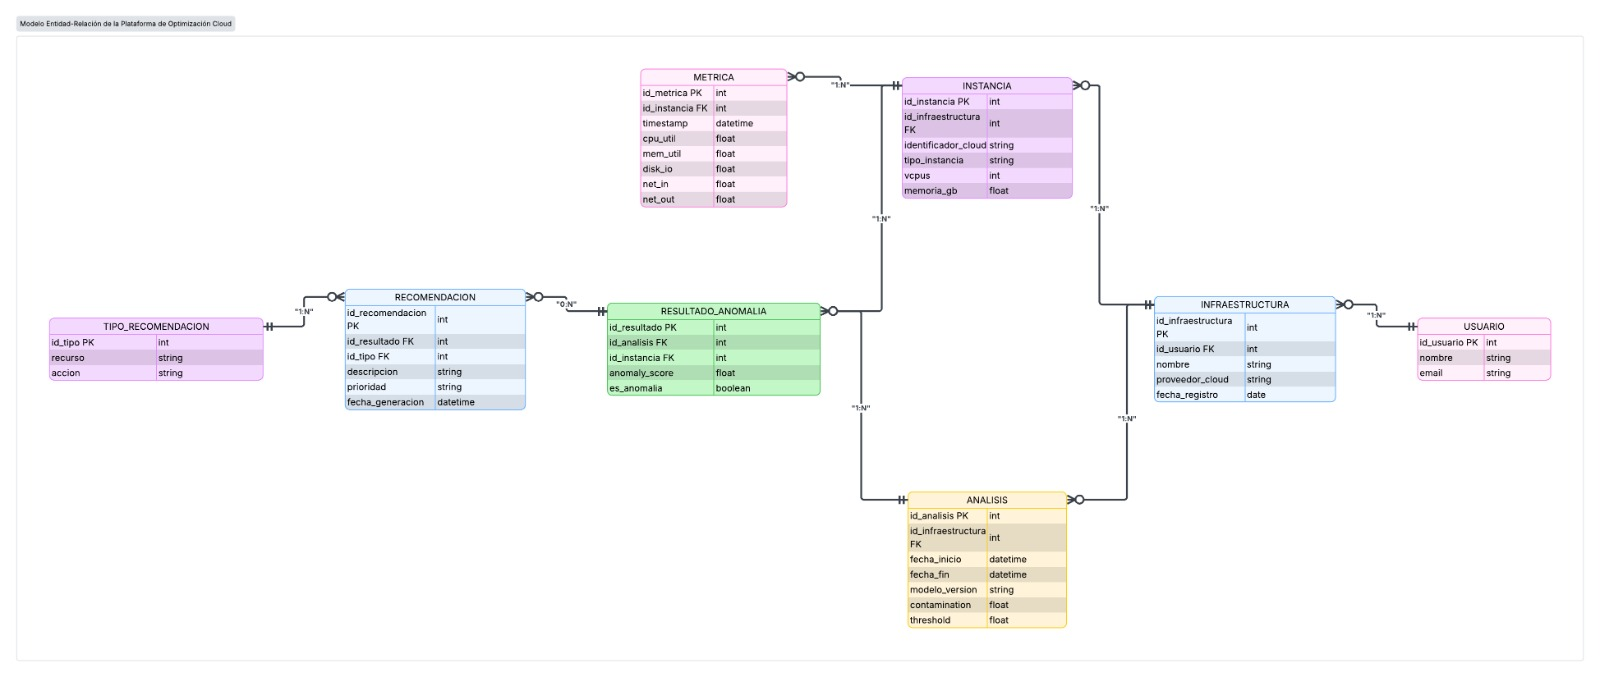
\includegraphics[width=8.48837in,height=2.37535in]{media/image2.png}

\hl{Figura 1: Cronograma, Diagrama de Gantt.}
\end{quote}

\end{document}
